%
% $Id: SANDExampleReportstrict.tex,v 1.28 2009-05-01 20:59:19 rolf Exp $
%
% This is an example LaTeX file which uses the SANDreport class file.
% It shows how a SAND report should be formatted, what sections and
% elements it should contain, and how to use the SANDreport class.
% It uses the LaTeX report class and the strict option.
%
% Get the latest version of the class file and more at
%    http://www.cs.sandia.gov/~rolf/SANDreport
%
% This file and the SANDreport.cls file are based on information
% contained in "Guide to Preparing {SAND} Reports", Sand98-0730, edited
% by Tamara K. Locke, and the newer "Guide to Preparing SAND Reports and
% Other Communication Products", SAND2002-2068P.
% Please send corrections and suggestions for improvements to
% Rolf Riesen, Org. 9223, MS 1110, rolf@cs.sandia.gov
%
% \documentclass[pdf,ps2pdf,12pt,report,strict,blank,OUO]{SANDreport}
\documentclass[pdf,ps2pdf,12pt,report,strict,blank]{SANDreport}
\usepackage{pslatex}
\usepackage{mathptmx}	% Use the Postscript Times font
\usepackage[FIGBOTCAP,normal,bf,tight]{subfig}
\usepackage{listings}
% \usepackage{enumitem}
% \usepackage{placeins}
\usepackage{caption}
% \usepackage{draftwatermark}
% \SetWatermarkScale{.5}
% \SetWatermarkText{\shortstack{Draft \\[1em] Contains OUO}}
% \SetWatermarkText{\shortstack{Draft}}

% If you want to relax some of the SAND98-0730 requirements, use the "relax"
% option. It adds spaces and boldface in the table of contents, and does not
% force the page layout sizes.
% e.g. \documentclass[relax,12pt]{SANDreport}
%
% You can also use the "strict" option, which applies even more of the
% SAND98-0730 guidelines. It gets rid of section numbers which are often
% useful; e.g. \documentclass[strict]{SANDreport}
\usepackage{graphicx}
\usepackage[table,xcdraw]{xcolor}

\definecolor{dkgreen}{rgb}{0,0.6,0}
\definecolor{gray}{rgb}{0.5,0.5,0.5}
\definecolor{mauve}{rgb}{0.58,0,0.82}


% ---------------------------------------------------------------------------- %
%
% Set the title, author, and date
%
    \title{SST-GPU: An Execution-Driven \\CUDA Kernel Scheduler and Streaming-Multiprocessor \\Compute Model}

    \author{M. Khairy$^1$, M. Zhang$^1$, R. Green$^1$,\\
            S. Hammond$^2$, R.J. Hoekstra$^2$, T. Rogers$^1$, and C. Hughes$^2$ \\
            \small{$^1$AALP Research Group, Purdue University, West Lafayette, IN 47907} \\
            \small{$^2$Center for Computing Research, Sandia National Laboratories, Albuquerque, NM 87185} \\
           }

%    \author{M. Khairy$^1$, M. Zhang$^1$, R. Green$^1$, T. Rogers$^1$,\\
%            S. Hammond$^2$, R.J. Hoekstra$^2$, and C. Hughes$^2$ \\
%            \small{$^1$AALP Research Group, Purdue University, West Lafayette, IN 47907} \\
%            \small{$^2$Center for Computing Research, Sandia National Laboratories, Albuquerque, NM 87185} \\
%           }

    % There is a "Printed" date on the title page of a SAND report, so
    % the generic \date should generally be empty.
    \date{}


% ---------------------------------------------------------------------------- %
% Set some things we need for SAND reports. These are mandatory
%
\SANDnum{SAND2019-1967}
\SANDprintDate{\today}
\SANDauthor{M. Khairy, M. Zhang, R. Green, and T. Rogers \\
            Accelerator Architecture Lab \\
            Purdue University \\
            West Lafayette, IN 47907 \\
            \parbox{6.5in}{khairy2011@gmail.com, zhan2308@purdue.edu, rgreen.dev@gmail.com, timrogers@purdue.edu} \\
            \\
            S.D. Hammond, R.J. Hoekstra, and C. Hughes \\
            Center for Computing Research \\
            Sandia National Laboratories \\
            Albuquerque, NM 87185 \\
            \{sdhammo, rjhoeks, chughes\}@sandia.gov
            }

% ---------------------------------------------------------------------------- %
% Include the markings required for your SAND report. The default is "Unlimited
% Release". You may have to edit the file included here, or create your own
% (see the examples provided).
%
% \include{MarkUR} % Not needed for unlimted release reports


% ---------------------------------------------------------------------------- %
% The following definition does not have a default value and will not
% print anything, if not defined
%
% \SANDsupersed{SAND1901-0001}{January 1901}
% \input{MarkOUO}


% ---------------------------------------------------------------------------- %
% Adjust floats
%
\setlength{\textfloatsep}{+18pt}
\setlength\abovecaptionskip{-6pt}

% ---------------------------------------------------------------------------- %
%
% Start the document
%
\begin{document}
    \maketitle

    % ------------------------------------------------------------------------ %
    % An Abstract is required for SAND reports
    %
    \begin{abstract}
	Programmable accelerators have become commonplace in modern computing systems.
Advances in programming models and the availability of massive amounts of data
have created a space for massively parallel acceleration where the context for
thousands of concurrent threads are resident on-chip. These threads are grouped
and interleaved on a cycle-by-cycle basis among several massively parallel
computing cores. The design of future supercomputers relies on an ability to
model the performance of these massively parallel cores at scale.

To address the need for a scalable, decentralized GPU model that can model large
GPUs, chiplet-based GPUs and multi-node GPUs, this report details the first
steps in integrating the open-source, execution driven GPGPU-Sim into the SST
framework. The first stage of this project, creates two elements: a kernel
scheduler SST element accepts work from SST CPU models and schedules it to an
SM-collection element that performs cycle-by-cycle timing using SST’s
MemHierarchy to model a flexible memory system.
%Initial results indicate a close
%correlation between the new GPU-SST model and real hardware.

    \end{abstract}


    % ------------------------------------------------------------------------ %
    % An Acknowledgement section is optional but important, if someone made
    % contributions or helped beyond the normal part of a work assignment.
    % Use \section* since we don't want it in the table of context
    %
    \clearpage
       \chapter*{Acknowledgment}
    We would like to thank Gwen Voskuilen for her help with MemHierarchy
and recommendations on debugging problems with the NIC and
interconnect. We would also like to thank Arun Rodrigues and 
Scott Hemmert for their support and help in defining the scope of the project.




    % ------------------------------------------------------------------------ %
    % The table of contents and list of figures and tables
    % Comment out \listoffigures and \listoftables if there are no
    % figures or tables. Make sure this starts on an odd numbered page
    %
    \cleardoublepage		% TOC needs to start on an odd page
    \tableofcontents
    \listoffigures
%     \listoftables


    % ---------------------------------------------------------------------- %
    % An optional preface or Foreword
%     \clearpage
%     \chapter*{Preface}
%     \addcontentsline{toc}{chapter}{Preface}
% 	\input{CommonPreface}


    % ---------------------------------------------------------------------- %
    % An optional executive summary
%     \clearpage
%     \chapter*{Summary}
%     \addcontentsline{toc}{chapter}{Summary}
% 	\input{CommonSummary}


    % ---------------------------------------------------------------------- %
    % An optional glossary. We don't want it to be numbered
    \clearpage
%     \chapter*{Nomenclature}
%     \addcontentsline{toc}{chapter}{Nomenclature}
%     \begin{description}
%     \end{description}


    % ---------------------------------------------------------------------- %
    % This is where the body of the report begins; usually with an Introduction
    %
    \SANDmain		% Start the main part of the report

   \chapter{Introduction}
      \label{Intro}
      With the rise of General-Purpose Graphics Processing Unit (GPGPU) computing and
compute-heavy workloads like machine-learning, compute accelerators have become
a necessary component in both high-performance supercomputers and
datacenter-scale systems. The first exascale machines are expected to heavily
leverage the massively parallel compute capabilities of GPUs or other highly
parallel accelerators \cite{snl_roadmap}. As the software stack and programming model of GPUs and
their accelerator peers continue to improve, there is every indication that
this trend will continue. As a result, architects that wish to study the design
of large-scale systems will need to evaluate the effect that their techniques have
using a GPU model. However, the focus of all publicly available cycle-level
simulators ({\em e.g}GPGPU-Sim \cite{gpgpu_sim}) to date, has been on single-node
simulation performance. In order to truly study
the problem at scale, or for the simulation of large workloads, a parallelizable,
multi-node GPU simulator is necessary.

   \begin{figure}[!htb]
      \centering
      \setlength{\abovecaptionskip}{6pt plus 1pt minus 1pt}
      \includegraphics[width=.85\textwidth,keepaspectratio]{figures/cpu_gpu_model.pdf}
      \captionsetup{width=.75\textwidth}
      \caption{High-level CPU/GPU interaction model}
      \label{fig:model}
   \end{figure}

Figure~\ref{fig:model} depicts the current CPU/GPU model co-processor model.
On the left is the common high-performance, discrete GPU configuration, where the CPU
and GPU have separate memory spaces and are connected via either PCIe or a
high-bandwidth link (such as NVLink). The right shows an Accelerated Processing Unit (APU
 model where the CPU
and GPU share a single memory. Note that in even in the discrete memory case, modern
memory translation units allow the CPU and GPU to share the same virtual address space,
although the memories themselves are discrete components.

In this report we will detail a model that is capable of simulating both
discrete and unified memory spaces by leveraging the MemHeirarchy interface in
SST \cite{sst}. This report details our efforts to integrate the functional and streaming
multiprocessor core models from the open-source simulator GPGPU-Sim into SST.


   \chapter{Scheduler Component}
      \label{sec:sched-comp}
      Table \ref{tab:apis} enumerates the CUDA API calls regarding to UVM currently supported by UVM Smart. These calls are enough to enable the execution of shared virtual memory space programming model. UVM Smart mainly adds on the modeling of far-fault handling latency and PCI-e transfer latency. Based on the Table \ref{tab:pcie}, a function to express PCI-e bandwidth as a function of transfer size is deducted. In the simulator, PCI-e transfer latency is calculated based on this expression.  an additional 100 core cycles for page table walk. The simulator makes simplified assumptions to model TLB and page table. The TLB look up is performed in a single core cycle based on the assumption of fully-associative TLB. A multi-threaded model for page table walk is used and an additional fixed 100 core cycles for page table walk is considered.

    \begin{table}[!htbp]
        \centering
        \setlength{\abovecaptionskip}{6pt plus 1pt minus 1pt}
        \captionsetup{width=.75\textwidth}
        \caption {CUDA API Calls Supported by UVMSmart.}
            \begin{tabular}{|l|l|c|}
                \hline
                \textbf{Transfer Size (KB)} & \textbf{PCI-e Bandwidth (GB/s)} \\
                \hline
                4 & 3.2219 \\
                \hline
                16 & 6.4437 \\ 
                \hline
                64 & 8.4771  \\
                \hline
	        256 & 10.508  \\
                \hline
		1024 & 11.223  \\
                \hline
            \end{tabular}
        \label{tab:pcie}
    \end{table}

    \begin{table}[!htbp]
        \centering
        \setlength{\abovecaptionskip}{6pt plus 1pt minus 1pt}
        \captionsetup{width=.75\textwidth}
        \caption {CUDA API Calls Supported by UVMSmart.}
            \begin{tabular}{|l|c|c|}
                \hline
                CUDACall  \\
                \hline
                \hline
                \texttt{cudaMallocManaged}  \\
                \hline
                \texttt{cudaDeviceSynchronize}  \\
                \hline
                \texttt{cudaMemprefetchAsync}  \\
                \hline
            \end{tabular}
        \label{tab:apis}
    \end{table}
    
The first step in merging UVMSmart into GPGPU-Sim is to understand the difference between them. Since UVMSmart extended GPGPU-Sim v3.2, the major change is a new class, called \texttt{gmmu\_t}, that handles the gpu memory management added to UVMSmart. This class stores necessary information about memory requests from all shader cores that missed in TLB. Then it figures out whether there is page-fault by looking up the page table. If page-fault, it would coalesce faults to the same page and handle these page faults one by one. If hardware prefetched is enabled, it would bring extra pages to GPU memory in the light of prefetching algorithms(Section B.4). And the update from GPGPU-Sim v3.2 to v4.0 has some minor changes, like making simulation cycle count a class variable instead of a global variable. Such minor changes would cause simulation crashes if not noticed and changed properly.

Table \ref{tab:uvm_tests} lists the number of benchmarks from various benchmark suites (Rodinia, Parboil, Lonestar, Parboil, HPC Challenge) that modified to use UVM.

    \begin{table}[!htbp]
        \centering
        \setlength{\abovecaptionskip}{6pt plus 1pt minus 1pt}
        \captionsetup{width=.75\textwidth}
        \caption {UVM Smart benchmarks}
            \begin{tabular}{|l|c|c|}
                \hline
                \textbf{Benchmark} & \textbf{Input} &  \textbf{Output}\\
                \hline
                bfs &  4096 & \\
                \hline
                hotspot & 30 6 40 & \\
                \hline
                pathfinder & 1000 20 5 & \\
                \hline
                backprop & 65536 & \\
                \hline
                srad & 1024 127 .5 4 & \\
                \hline
            \end{tabular}
        \label{tab:uvm_tests}

    \end{table}

 The configuration for the GPGPU Simulator supporting Unified Virtual Memory is shown in Listing \ref{lst:sst_config}.


\lstdefinelanguage{mooCows}
{
  basicstyle={\small\ttfamily},
  columns=flexible,
  tag=[s]{[]},
  tagstyle=\color{dkgreen}\bfseries,
  usekeywordsintag=true
}[html]

\lstset{frame=tb,
  language=mooCows,
  aboveskip=3mm,
  belowskip=3mm,
  showstringspaces=false,
  columns=flexible,
  basicstyle={\small\ttfamily},
  numbers=none,
  numberstyle=\tiny\color{gray},
  breaklines=true,
  breakatwhitespace=true,
  tabsize=3
}

\lstinputlisting[caption=Sample GPGPU-Sim UVM Smart Configuration, label=lst:sst_config]{figures1/config}



   \chapter{Streaming-Multiprocessor Component}
      \label{sec:sm-comp}
      To support the GPGPU-Sim functional model, a number of the simulator's overloaded
CUDA Runtime API calls were updated. Several functions that originally assumed
the application and simulator were within the same address space now support them being
decoupled. Initialization functions, such as \texttt{\textunderscore \textunderscore
cudaRegisterFatBinary}, now take paths to the original application to obtain the PTX
assembly of CUDA kernels.


   \begin{figure}[!htb]
      \centering
      \setlength{\abovecaptionskip}{6pt plus 1pt minus 1pt}
      \includegraphics[width=.90\textwidth,keepaspectratio]{figures/transfer_flow.eps}
      \captionsetup{width=.75\textwidth}
      \caption{Data transfer flow for functional simulation}
      \label{fig:gpu_transfer_model}
   \end{figure}

Supporting the functional model of GPGPU-Sim also requires transferring values
from the CPU application to the GPU memory system. This is solved by leveraging
the link between CPU/GPU and memory hierarchy from SST, as shown in
\ref{fig:gpu_transfer_model}. Data are transferred from the application to Ariel through
inter-process communication tunnels. Ariel then communicates with the GPU scheduler through
the CPU memory. The GPU scheduler then writes the data to the GPU memory. When an SM
requests a piece of data, the SM accesses the GPU memory for it.
The tunnels utilize 4KiB size as the granularity, while CPU and GPU components
employ larger size non-cacheable requests to access to CPU and GPU memories.

To model GPU performance, the memory system of the public GPGPU-Sim is
completely removed. Instead, all accesses to GPU memory are sent though SST
links to the MemHierarchy interface. As Figure \ref{fig:gpu_mem_model} shows, a
multi-level cache hierarchy is simulated with the shared L2 sliced between
different memory partitions, each with its own memory controller. Several
backend timing models have been configured and tested, including SimpleMem,
SimpleDRAM, TimingDRAM, and CramSim \cite{healy2017}; CramSim will be used to
model the HBM stacks in the more detailed performance models. We have created an
initial model for the GPU system similar to that found in an Nvidia Volta. The
configuration for the GPU, CramSim and Network components is shown in Listing
\ref{lst:sst_config}.


\lstdefinelanguage{mooCows}
{
  basicstyle={\small\ttfamily},
  columns=flexible,
  tag=[s]{[]},
  tagstyle=\color{dkgreen}\bfseries,
  usekeywordsintag=true
}[html]

\lstset{frame=tb,
  language=mooCows,
  aboveskip=3mm,
  belowskip=3mm,
  showstringspaces=false,
  columns=flexible,
  basicstyle={\small\ttfamily},
  numbers=none,
  numberstyle=\tiny\color{gray},
  breaklines=true,
  breakatwhitespace=true,
  tabsize=3
}

\lstinputlisting[caption=Sample SST-GPGPU Configuration, label=lst:sst_config]{figures/config}
\clearpage


%    \chapter{Evaluation}
%       To evaluate the performance correlation of our GPU-SST model, versus both real
hardware and the existing GPGPU-Sim memory system implementation an execution
time correlation is done on the vectorAdd benchmark from the CUDA SDK. Figure
\ref{fig:titanv_result} shows the results of this timing analysis. The most
accurate GPGPU-Sim timing model is reasonably accurate (within 25\% of the
hardware results), however GPU-SST is much closer to real hardware, showing
just and 8\% deviation from a silicon Nvidia Titan V card.


   \begin{figure}[!htb]
      \centering
      \setlength{\abovecaptionskip}{6pt plus 1pt minus 1pt}
      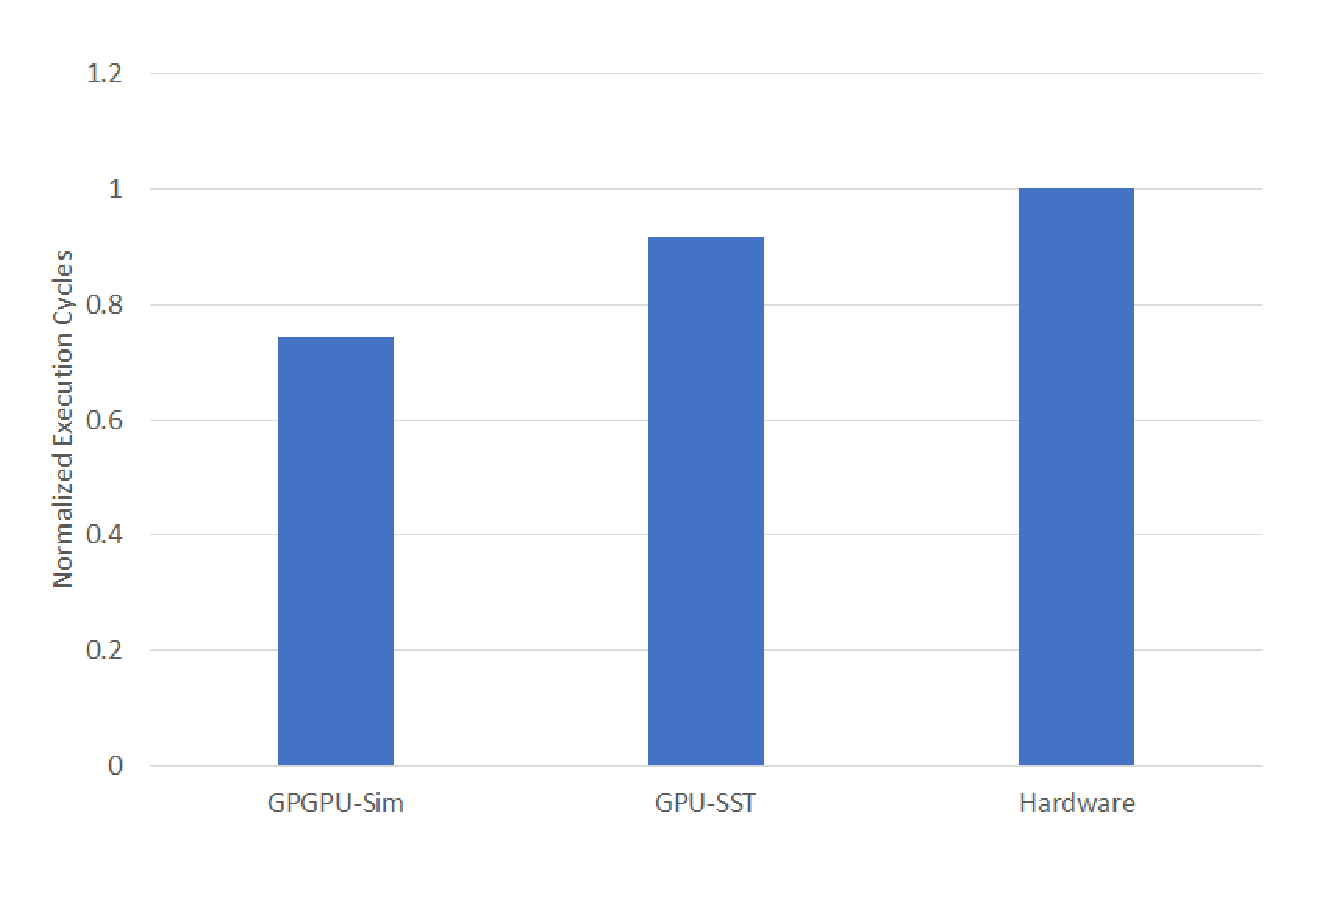
\includegraphics[width=.50\textwidth,keepaspectratio]{figures/4_1.eps}
      \captionsetup{width=.90\textwidth}
      \caption{Normalized execution time for 160k element vector addition kernel -- \\
               SST-GPU is within 8\% of the silicon of the Titan V}
      \label{fig:titanv_result}
   \end{figure}


   \chapter{Conclusion}
      This report has detailed the first phase of the SST-GPU project, where the
execution-driven functional and performance model of a GPU had been integrated
SST. Initial results demonstrate significant coverage of applications. The next phase of the project will
focus on further disaggregating the GPU to enable truly scaled GPU performance
in a multi-process MPI simulation.


    \nocite{*}


    % ---------------------------------------------------------------------- %
    % References
    %
    \clearpage
    % If hyperref is included, then \phantomsection is already defined.
    % If not, we need to define it.
    \providecommand*{\phantomsection}{}
    \phantomsection
    \addcontentsline{toc}{chapter}{References}
    \bibliographystyle{plain}
    \bibliography{sst_gpgpu_bib}


    % ---------------------------------------------------------------------- %
    %
%     \appendix
%     \chapter{Historical Perspective}
% 	\input{CommonHistory}
%
%
%     \chapter{Some Other Appendix}
% 	\input{CommonAppendix}

    % \printindex

    \include{SANDdistribution}


\end{document}
